\documentclass[../ComplexAnalysis_Notes.tex]{subfiles}

\begin{document}
\chapter*{Lecture 4} %Set chapter name
\addcontentsline{toc}{chapter}{Lecture 4} %Set chapter title

\setcounter{chapter}{4} %Set chapter counter
\setcounter{section}{0}
\setcounter{equation}{0}
\setcounter{figure}{0}

 \section{Cauchy Integral Theorem}

 Last day we have seen, if a function have primitive over a simply connected domain, its' integral over the boundary of that region is 0. We also noted for a function $\frac{1}{z}$, integration (countour integral) over $\partial B_{r}(0)$ is not zero.  So, it can't have a primitive over the region $\C \setminus \qty{0}$. The function is Holomorphic on any open set do not contain $0$. So the natural question arises,`Is it possible that, this function has primitive in some open set do not contain $0$?' To answer this question we need `Cauchy Integral Theorem', which is stated as following. 

 \begin{Thm}{Cauchy(Goursat) Integral Theorem}{}
    \hspace*{0.1cm} Let, $f \in  \Hol(\mathcal{O})$, where $\mathcal{O}$ is simply connected domain. Then, $\int_{\gamma} f dz\, =0$ for all piece-wise smooth closed curve $\gamma \subset \mathcal{O}$. 
 \end{Thm}

\noindent To prove this we need to develop more techniques in complex analysis. Rather, we will prove a weak version of the above theorem. 

\begin{Thm}{Cauchy Integral Theorem $\Delta$ version}{} \label{thm:4.1}
    \hspace*{0.1cm} Let, $\gamma$ is a triangle (curve including sides of the triangle $T$) and $\operatorname{int}(T) \cup T \subseteq \mathcal{O}$. Then for all $f \in \Hol(\mathcal{O})$, \[
        \int_{T} f dx\, = 0
    \]     
\end{Thm}

\begin{wrapfigure}{r}{0mm}
    \centering
     

\tikzset{every picture/.style={line width=0.75pt}} %set default line width to 0.75pt        

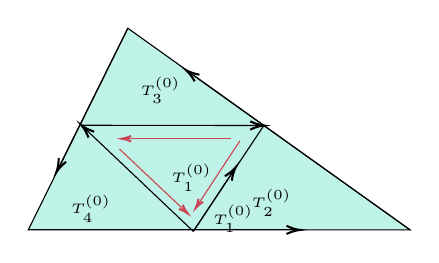
\begin{tikzpicture}[x=0.75pt,y=0.75pt,yscale=-1,xscale=1]
%uncomment if require: \path (0,300); %set diagram left start at 0, and has height of 300

%Shape: Triangle [id:dp19363273338874776] 
\draw  [fill={rgb, 255:red, 192; green, 243; blue, 232 }  ,fill opacity=1 ] (299,103.27) -- (435,200.44) -- (251,200.44) -- cycle ;
%Straight Lines [id:da13369882424805235] 
\draw    (299,103.27) -- (265.43,170.85) ;
\draw [shift={(264.54,172.64)}, rotate = 296.41] [color={rgb, 255:red, 0; green, 0; blue, 0 }  ][line width=0.75]    (6.56,-1.97) .. controls (4.17,-0.84) and (1.99,-0.18) .. (0,0) .. controls (1.99,0.18) and (4.17,0.84) .. (6.56,1.97)   ;
%Straight Lines [id:da7026867637204568] 
\draw    (435,200.44) -- (328.63,124.6) ;
\draw [shift={(327,123.44)}, rotate = 35.49] [color={rgb, 255:red, 0; green, 0; blue, 0 }  ][line width=0.75]    (6.56,-1.97) .. controls (4.17,-0.84) and (1.99,-0.18) .. (0,0) .. controls (1.99,0.18) and (4.17,0.84) .. (6.56,1.97)   ;
%Straight Lines [id:da24532905932049798] 
\draw    (251,200.44) -- (380,200.44) ;
\draw [shift={(382,200.44)}, rotate = 180] [color={rgb, 255:red, 0; green, 0; blue, 0 }  ][line width=0.75]    (6.56,-1.97) .. controls (4.17,-0.84) and (1.99,-0.18) .. (0,0) .. controls (1.99,0.18) and (4.17,0.84) .. (6.56,1.97)   ;
%Straight Lines [id:da7720971354083273] 
\draw    (276.65,150.02) -- (362.54,150.14) ;
\draw [shift={(364.54,150.14)}, rotate = 180.08] [color={rgb, 255:red, 0; green, 0; blue, 0 }  ][line width=0.75]    (6.56,-1.97) .. controls (4.17,-0.84) and (1.99,-0.18) .. (0,0) .. controls (1.99,0.18) and (4.17,0.84) .. (6.56,1.97)   ;
%Straight Lines [id:da8065003073856949] 
\draw    (330.54,201.14) -- (278.1,151.4) ;
\draw [shift={(276.65,150.02)}, rotate = 43.49] [color={rgb, 255:red, 0; green, 0; blue, 0 }  ][line width=0.75]    (6.56,-1.97) .. controls (4.17,-0.84) and (1.99,-0.18) .. (0,0) .. controls (1.99,0.18) and (4.17,0.84) .. (6.56,1.97)   ;
%Straight Lines [id:da0969029289851786] 
\draw    (330.54,201.14) -- (364.54,150.14) ;
%Straight Lines [id:da4256536754887119] 
\draw    (330.54,201.14) -- (349.94,171.81) ;
\draw [shift={(351.04,170.14)}, rotate = 123.48] [color={rgb, 255:red, 0; green, 0; blue, 0 }  ][line width=0.75]    (6.56,-1.97) .. controls (4.17,-0.84) and (1.99,-0.18) .. (0,0) .. controls (1.99,0.18) and (4.17,0.84) .. (6.56,1.97)   ;
%Straight Lines [id:da872485784840215] 
\draw [color={rgb, 255:red, 204; green, 68; blue, 84 }  ,draw opacity=1 ]   (348.5,156.5) -- (298.22,156.5) ;
\draw [shift={(296.22,156.5)}, rotate = 360] [color={rgb, 255:red, 204; green, 68; blue, 84 }  ,draw opacity=1 ][line width=0.75]    (4.37,-1.32) .. controls (2.78,-0.56) and (1.32,-0.12) .. (0,0) .. controls (1.32,0.12) and (2.78,0.56) .. (4.37,1.32)   ;
%Straight Lines [id:da9572567764244801] 
\draw [color={rgb, 255:red, 204; green, 68; blue, 84 }  ,draw opacity=1 ]   (295,161.5) -- (326.27,191.03) ;
\draw [shift={(327.72,192.4)}, rotate = 223.36] [color={rgb, 255:red, 204; green, 68; blue, 84 }  ,draw opacity=1 ][line width=0.75]    (4.37,-1.32) .. controls (2.78,-0.56) and (1.32,-0.12) .. (0,0) .. controls (1.32,0.12) and (2.78,0.56) .. (4.37,1.32)   ;
%Straight Lines [id:da5946970805491989] 
\draw [color={rgb, 255:red, 204; green, 68; blue, 84 }  ,draw opacity=1 ]   (353,157.5) -- (332.82,188.17) ;
\draw [shift={(331.72,189.84)}, rotate = 303.35] [color={rgb, 255:red, 204; green, 68; blue, 84 }  ,draw opacity=1 ][line width=0.75]    (4.37,-1.32) .. controls (2.78,-0.56) and (1.32,-0.12) .. (0,0) .. controls (1.32,0.12) and (2.78,0.56) .. (4.37,1.32)   ;

% Text Node
\draw (319,167.4) node [anchor=north west][inner sep=0.75pt]  [font=\tiny]  {$T_{1}^{( 0)}$};
% Text Node
\draw (357.5,179.4) node [anchor=north west][inner sep=0.75pt]  [font=\tiny]  {$T_{2}^{( 0)}$};
% Text Node
\draw (304,125.4) node [anchor=north west][inner sep=0.75pt]  [font=\tiny]  {$T_{3}^{( 0)}$};
% Text Node
\draw (339,187.4) node [anchor=north west][inner sep=0.75pt]  [font=\tiny]  {$T_{1}^{( 0)}$};
% Text Node
\draw (270.5,182.4) node [anchor=north west][inner sep=0.75pt]  [font=\tiny]  {$T_{4}^{( 0)}$};


\end{tikzpicture}
  
\end{wrapfigure}

\vspace*{0.1cm}

\noindent \textit{Proof.} Lat, $T^{0}$ b the curve $T$ with anticlockwise direction. Take the middle point of each side and joint them to get $4$ triangles (as shown in the picture) with an orientation (shown in the picture). Call these triangles $T^{(0)}_j$ for $j=1,\cdots,4$.

\vspace*{0.2cm}

\noindent Let, $I  = \int_{T^{(0)}} f dz\,$. From the above partition we can say, \begin{align*}
    & I = \int_{T^{(0)}} f dz\, = \sum_{j=1}^4 \int_{T^{(0)}_j} f dz\, \\
    & \abs{I} \leq \sum_{j=1}^4 \abs{\int_{T^{(0)}_j} f dz\,} \leq  4 \abs{\int_{T^{(0)}_i} f dz\,}
\end{align*}

\vspace*{0.2cm}

The last inequality holds for some $i \in \qty{1,2,3,4}$. Now call this triangle $T^{(0)}_i:= T^(1)$. We carry out the calculations for $i =1,\cdots,n$ and obtain $\frac{1}{4^n} \abs{I} \leq \abs{\int_{T^{(n)}} f dz\,}$. Set, $\mathcal{T}^{(n)} := T^{(n)} \cup \operatorname{int} (T^{(n)})$. These sets are compact for $n \in \N$. Thus, we have a chain of compact (closed subsets), $$\mathcal{T}^{(0)} \supset \mathcal{T}^{(1)} \supset \cdots$$
with  $\operatorname{diam} \mathcal{T}^{(n)} = \frac{1}{2^n} \operatorname{diam} \mathcal{T}^{(0)}= \frac{1}{2^n}(\text{ length of largest side of }  \mathcal{T}^{(0)})$. Using ``\textbf{Cantor intersection theorem}'' we get, $$\bigcap_{n=0}^{\infty} \mathcal{T}^{(n)} = \qty{z_0}\, (\text{singleton set})$$
Using holomorphic property of $f$ at $z_0$ we get, $f(z)= f(z_0)+f'(z_0)(z-z_0)+R(z)(z-z_0)$ holds in some open ball $B_{\epsilon}(z_0)$ around $z_0$, where $R(z)$ is continuous on that open ball with $\lim R(z) =0$ as $z \to z_0$. Take $n$ large enough so that $\mathcal{T}^{(n)}\subset B_{\epsilon}(z_0)$.
\begin{align*}
    \int_{T^{(n)}} f dz\, &= \int_{T^{(n)}} \qty[f(z_0)+f'(z_0)(z-z_0) +R(z)(z-z_0)] dz\,\\
    &= \int_{T^{(n)}} R(z)(z-z_0) dz\, \\
    \implies \frac{1}{4^n}\abs{I} &\leq \abs{\int_{T^{(n)}} R(z)(z-z_0) dz\,}
\end{align*}
Set, $\epsilon_n := \sup_{z \in T^{(n)}}\abs{R(z)}$. Note that as $n \to \infty$, $\epsilon_n \to 0$. Also, for $z \in \mathcal{T}^{(n)}$ we have, $\abs{z-z_0} \leq \operatorname{diam} \mathcal{T}^{(n)} = \frac{1}{2^n}d_0$ (here, $d_0$ is the length largest side of $T^{(n)}$). Using triangle inequality we get, \begin{align*}
    \frac{1}{4^n} \abs{I} &\leq  \abs{\int_{T^{(n)}}R(z)(z-z_0)\, dz} \leq \sup_{z \in T^{(n)}} \abs{R(z)} \times \frac{d_0}{2^n} \times \operatorname{len}(T^{(n)})\\
    &= \frac{3d_0}{4^n} \cdot \epsilon_n\\
    \abs{I} &\leq 3d\epsilon_n
\end{align*}
Just by taking the limit $n \to \infty$ we have $I =0$. $\hfill \blacksquare$

\vspace*{0.2cm} %coro

\hspace*{0.6cm} \textcolor{violet}{\textsc{Corollary}.} \textit{If $R$ is a rectangle $R \subset \mathcal{O}$ and $f \in \Hol (\mathcal{O})$, then $\int_{R} f dz\,=0$.}

\vspace*{0.1cm}

\noindent Now we will look at the question, we concerned at the beginning. `Does the primitive of $\frac{1}{z}$ exist in some domain $0 \notin B_{\epsilon}(z_0)$?' The answer is \textbf{Yes}! It should be given by $g(z) := \int_{\gamma_z} f\, dz$ where $\gamma_z$ is a path from $z_0$ to $z$.  The natural question should be to prove the well define-ness of the above $g$. We have to show, no matter what path b/w $z$ and $z_0$ we choose, value of $g(z)$ must be same. If we have proven \textbf{main Cauchy theorem} then for any two path $\gamma,\eta$ (that do not intersect each other except the end points) joining $z$ and $z_0$, we will consider the concatenated loop $\gamma \ast \eta^{-1}$. Since the disc is simply-connected, the region bounded by the loop is also simply connected.Thus the theorem gives, $\int_{\gamma \ast \eta^{-1}} f \, dz =0$ which gives $\int_{\gamma} f = - \int_{\eta^{-1}} f\, dz = \int_{\eta} f\, dz$. Thus, the function we defined is well-defined. Since we haven't proved the strong Cauchy theorem, we will answer the question with the help of following theorem. 

\begin{Thm}{}{}\label{thm:4.2}
    \hspace*{0.1cm} Let, $\mathcal{U} \subseteq \mathcal{O}$ open and convex.  $f \in \operatorname{Cont}(\mathcal{U})$ and suppose $\int_{\Delta} f \, dz =0$ for all $\Delta \subseteq \mathcal{U}$. Fix $z_0 \in \mathcal{U}$ and let $[z_0,z]$ be the line joining $z_0$ to $z$.  Define, \[g(z):= \int_{[z_0,z]}f\, dz \]
    Then $g \in \Hol (\mathcal{U})$ and $g^{\prime} =f$.
\end{Thm}

\noindent \textit{Proof}. Fix $\tilde{z} \in \mathcal{U}$ and $T_{z}$ be the triangle with sides $[z_0,\tilde{z}],[\tilde{z},z], [z,z_0]$ (with this orientation). By the property of $f$ we can say, $\int_{T_z} f\, dz =0$. Expanding this integral we get, \begin{align*}
    & \Rightarrow \int_{[z_0,\tilde{z}]} f \, dz + \int_{[\tilde{z},z]} f \, dz + \int_{[z,z_0]} f \, dz =0 \\
    & \Rightarrow g(\tilde{z}) -g(z) =  \int_{[z,\tilde{z}]} f \, dz  \\
    &\Rightarrow \frac{g(z)-g(\tilde{z})}{z-\tilde{z}} = \frac{1}{z-\tilde{z}}  \int_{[z,\tilde{z}]} f \, dz  \\
    &\Rightarrow \abs{\frac{g(z)-g(\tilde{z})}{z-\tilde{z}}-f(\tilde{z})} =   \frac{1}{\abs{z-\tilde{z}}}\abs{\int_{[z,\tilde{z}]} f \, dz} 
\end{align*}
Using continuity of $f$ we can say RHS of the above equation is $<\epsilon$ in some open nbd around $\tilde{z}$. Thus, $g$ is holomorphic at $\tilde{z}$ with $f(\tilde{z})=g'(\tilde{z})$, we can do this for any $\tilde{z} \in \mathcal{U}$ and hence we are done. $\hfill \blacksquare$

\vspace*{0.2cm} %coro

\hspace*{0.6cm} \textcolor{violet}{\textsc{Corollary}.} \textit{Let, $f\in \Hol (\mathcal{U})$ (with $\mathcal{U}$ is open and convex). Then there exist $ g \in \Hol (\mathcal{U})$ such that $g'=f$ and $\int_{\gamma} f\, dz =0$ for all smooth piece-wise smooth loop $\gamma$ in $\mathcal{U}$.}


%%%%%%%%%%%%%%

\begin{center}
    ---------------------------------------------

    ``\textcolor{darkcerulean}{One big theorem at a day}''- \textit{JDS}
\end{center}

\end{document}